%!TEX root = ../report.tex
\chapter{Improving Automated Build}
For this sprint we choose to work on four user stories that we expect to improve automated building.

\begin{chapterorganization}
  \item In \sectionref{sec:jenkins_restruct} we explain how we restructure jobs in Jenkins to ease further configuration needs;
  \item in \sectionref{sec:s3_linecoverage} we enable generation of a code coverage report and show the result in the overview list in Jenkins;
  \item in \sectionref{sec:upload_google_play} we automatically upload successful builds to the Google Play alpha channel;
  \item in \sectionref{sec:monkey_testing_s2} we describe our work towards making monkey testing work;
  \item in \sectionref{sec:s3_appinstallationtest} we set up a test case that installs all apps on the same device to check if apps are compatible, since this has been an issue.
\end{chapterorganization}

\section{Restructuring Jenkins}\label{sec:jenkins_restruct}
The setup of Jenkins used in sprint 1 was tedious to work with since all jobs were configured independently. If a change had to be made to several jobs, we would have to manually configure the change in each job. Not only did this take a considerable amount of time, but it was also prone to human errors during the process. In this sprint, we predict that we will have make small modifications to all jobs several times. This would be very tedious, so we decide to make job configurations easier to manage, even though it is not connected directly to a story. We consider it refactoring.

The jobs in Jenkins are generally very similar in their configuration. We can benefit from having a base configuration, which the jobs only modify. There exists a Jenkins plug-in for this, called inheritance-plugin \parencite{jenkins-inheritance}. With this plug-in installed, whenever we decide to make a change to e.g.\ the build system, it will not be necessary to change this in each job. Instead, the change can be made on the base job, and all relevant jobs will inherit this change. This also ensures that jobs follow a consistent pipeline and thus do not differ from job to job.

The plug-in requires the jobs to be of a special \emph{inheritable} type. We therefore have to convert the existing jobs to inheritable jobs to take advantage of this. As an existing job cannot automatically be converted to the inheritable type, we have to re-create all the jobs. We do not consider this a concern, as the time to setup will be considerably shorter when taking advantage of the inheritable job type. When the old jobs are removed the build history will be lost. This is a minor nuisance but we consider it a small price to pay, compared to the advantages. When deciding how to structure the build, we see two general categories that are sufficiently distinct: \emph{Android Apps} and \emph{Android Libraries}. We create an abstract job for each of these. They do overlap somewhat in functionality, which means we have to create an abstract job for each build step. As such we create abstract jobs for e.g.\ \emph{Email}, \emph{Emulator}, and \emph{CoCo} (code coverage). The abstract jobs Android App and Android Library inherit from the small abstract jobs that are relevant. We have modeled this as a diagram in \figureref{fig:jenkins_inherit}.

\begin{figure}%
\centering
\tikzsetnextfilename{jenkins_inherit}
\begin{tikzpicture}[
  simple/.style={draw, rounded corners, minimum height=1.8em},
  simplefixed/.style={draw, rounded corners, minimum height=1.8em, minimum width=10em},
  square/.style={draw, rounded corners, minimum height=1.4em, minimum width=1.4em}]

  \begin{scope}[]
    \matrix[column sep=.5cm]{
      \node[simple] (pubAPK) {Publish APK}; &
      \node[simple] (email) {Email}; &
      \node[simple] (coco) {CoCo}; &
      \node[] (dots) {\dots};  &
      \node[simple] (emu) {Emulator}; &
      \node[simple] (pubLib) {Publish lib}; \\
    };
  \end{scope}

  \begin{scope}[yshift=-2cm]
    \matrix[column sep=1.5cm]{
      \node[simplefixed] (appInh) {Android App}; &
      \node[simplefixed] (libInh) {Android Library}; \\
    };
  \end{scope}

  \begin{scope}[yshift=-3.5cm]
    \matrix[column sep=.3cm]{
      \node[simple] (app1) {App 1}; &
      \node[simple, right=of app1] (app2) {App 2}; &
      \node[right=of app2] (dots) {\dots}; &
      \node[simple, right=of dots] (appn) {App $n$}; &
      \node[] (dummy) {}; &
      \node[] (dummy2) {}; &
      \node[simple] (lib1) {Lib 1}; &
      \node[simple, right=of lib1] (lib2) {Lib 2}; &
      \node[right=of lib2] (dots) {\dots}; &
      \node[simple, right=of dots] (libn) {Lib $n$}; \\
    };
  \end{scope}

  \draw[<-] (appInh) to (app1);
  \draw[<-] (appInh) to (app2);
  \draw[<-] (appInh) to (appn);
  \draw[<-] (libInh) to (lib1);
  \draw[<-] (libInh) to (lib2);
  \draw[<-] (libInh) to (libn);

  \draw[<-] (pubAPK) to (appInh);
  \draw[<-] (email) to (appInh);
  \draw[<-] (coco) to (appInh);
  \draw[<-] (emu) to (appInh);

  \draw[<-] (pubLib) to (libInh);
  \draw[<-] (email) to (libInh);
  \draw[<-] (coco) to (libInh);
  \draw[<-] (emu) to (libInh);

  \draw[decorate, line width=1pt, decoration={brace, mirror}] ([xshift=1.5em]pubLib.south east) -- ([xshift=1.5em]pubLib.north east) node [midway, yshift=0em, xshift=2.7em] {Sub-tasks};

  %\draw[decorate, line width=1pt, decoration={brace, mirror}] ([xshift=1.5em]bd.south east) -- ([xshift=1.5em]bd.north east) node [midway, yshift=-0.1em, xshift=3.2em] {Subprojects};

\end{tikzpicture}
\caption{Jenkins inheritable jobs}%
\label{fig:jenkins_inherit}%
\end{figure}

\section{Code Coverage Reports}\label{sec:s3_linecoverage}
We have a user story which states that Jenkins should provide code coverage metrics for every GIRAF project. This user story was suggested by a group who was writing tests for a database project and wanted a measure of their progress. Their main request is for a percentage of lines of code covered. A tool for code coverage report must at least provide this metric. In version 0.10 of the \emph{New Android SDK Build System} \parencite{new-build-android}, support for the JaCoCo \parencite{jacoco-home} Java Code Coverage Library was included. It meets all of our demands for metrics and is nicely integrated into the Android and Gradle build system. To make JaCoCo generate a report, we simply enable it in the \mono{build.gradle} file of the project.

Now we generate code coverage reports for debug builds locally and in Jenkins. We would also like to publish the code coverage results in Jenkins. There exists a Jenkins plugin \parencite{jacoco-jenkins-plugin} for this purpose. This plugin is easy to setup, provides detailed coverage statistics, and an overview with the percentage of lines of code covered. We use this plugin for publishing the code coverage metrics in Jenkins. An example of the Jenkins overview screen with code coverage metrics can be seen in \figureref{fig:jenkins-overview-coco}.

\begin{figure}[tbp]
    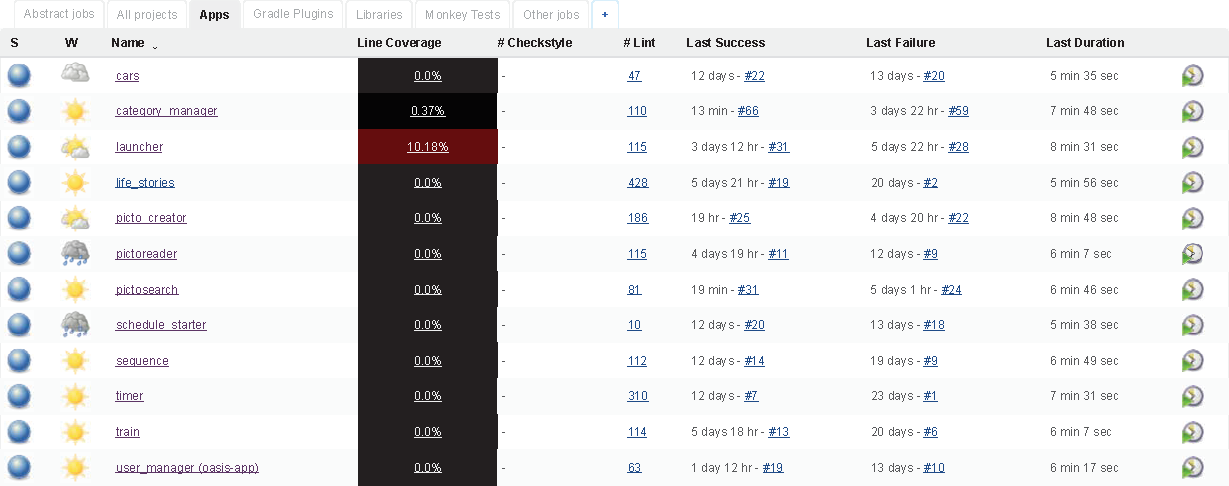
\includegraphics[width=\textwidth]{graphics/jenkins-overview-coco.pdf}
    \caption{Screenshot of a section of the build overview screen which shows the code coverage column}
    \label{fig:jenkins-overview-coco}
\end{figure}

\section{Upload of Apps to Google Play}\label{sec:upload_google_play}
Jenkins compiles and builds the GIRAF projects but does nothing with the generated APKs. One of the user stories selected in this sprint is \us{automatic upload of alpha releases to Google Play}.

Before the APKs can be published to Google Play, they need to be signed with a signature. The Android plugin for Gradle has functionality for automatic signing of APKs, and we will use this to sign. A keystore file is used to sign, and we are not interested in everybody having this file as it serves as a proof of identification. We save the file on the server, which means that it becomes impossible to build release versions of the apps locally. When uploading a new app to Google Play, the version code of the new app must be greater than the version code of the app already in the app store. Incrementing the version code is not done per default, so we need to set up the build to increase the version code every time an app is successfully built.

We have written a Gradle plugin handling this with the major part of this seen in \listingref{lst:gradle_versioncode}. The full plugin can be seen in \appendixref{app:gradle_plugins}. The plugin keeps a \mono{.properties} file with the current version code for all apps. Upon executing the \code{increaseVersionCode} Gradle task, it reads the version code (line \ref{gradlevs:8}) from the properties file and increments it (line \ref{gradlevs:12}). Then it writes it to the app manifest file, such that the build following will use the new version code. Finally, it updates the property file with the new version code, such that the next build will use this version code. If no current version code is found in the properties file, we assume the app is new and starts at version code \mono{1}, and as such we do not increment it.
\begin{gradlecode}[float=tbp,caption=Part of our Gradle plugin for updating version code (written in Groovy),label=lst:gradle_versioncode]
project.task('increaseVersionCode') << {
    // [...]
    // Check to see if properties file exists.
    if (project.file(versionCodesFilePath).exists() != true) {
        throw new GradleException("No version code file found. Only Jenkins should run this task")
    }
    // [...]
    def newVersion = getVersionCode(project, applicationId)(*@\label{gradlevs:8}@*)
    def versionCode = newVersion['value']
    if (!newVersion['created']) { (*@\label{gradlevs:10}@*)
        // Increment version code if not new
        versionCode++ (*@\label{gradlevs:12}@*)
        // Write incremented version code to manifest (*@\label{gradlevs:13}@*)
        // [...]
        // Write incremented version code back to properties file (*@\label{gradlevs:15}@*)
        // [...]
    }
}

def getVersionCode(project, applicationId) {
    // Reads the version code from the properties file. Returns 1 if the version code does not exist. (*@\label{gradlevs:21}@*)
}
\end{gradlecode}

Now that the APKs have been signed, they need to be uploaded to Google Play. This can be done in two ways: Via a Jenkins plugin \parencite{jenkins-play-plugin} or through Gradle \parencite{gradle-play-plugin}. The Jenkins plugin is easy to use, but requires that the exact name and location of the APK to upload is known. The Gradle plugin knows this already, since the information is already present in the Gradle build environment. Therefore we use Gradle to publish to Google Play via a Google Play API\@. After the APKs have been uploaded, they are moved to the FTP server which is hosted on the same machine as Jenkins in the directory \mono{/srv/ftp/}. This way the APKs are also available outside of the Google Play store.

\section{Monkey Testing}\label{sec:monkey_testing_s2}
During sprint 1 we encountered some difficulties related to monkey testing. In order to monkey test apps we need to install those apps on an Android device, but we did not have these apps easily available. As described in \sectionref{sec:upload_google_play} the signed APKs for each app is now stored on the FTP sever. As the FTP server is hosted on the same machine as Jenkins, we can directly access the APKs from the directory. To install we simply need to identify the newest build of each app, as, for now, the old builds are kept as well.

To find the APK for the newest version of a specific app, we use the script seen in \listingref{lst:find_newest_apk}, parsing to it the application id of the app. All APKs containing the given application id is then found. This result is piped to \code{sed 's/.*b//' | sed 's/\_release\_aligned.apk//'} that removes everything but the build number of the files. \code{awk '\$0>x\{x=\$0\};END\{print x\}'} \parencite{stackoverflow-max-number2012} then finds the maximum build number. Finally the path of the newest APK for the given application id is found.

For example, consider the following APK files:

\begin{lstlisting}[language=bash]
dk.aau.cs.giraf.launcher_v2.3b18_release_aligned.apk
dk.aau.cs.giraf.launcher_v2.3b19_release_aligned.apk
dk.aau.cs.giraf.launcher_v2.3b20_release_aligned.apk
dk.aau.cs.giraf.launcher_v2.3b21_release_aligned.apk
\end{lstlisting}

The APK with the highest build number is the newest. The build number is the number after the \code{b} in the file name. Running the script in \listingref{lst:find_newest_apk} with the application id \code{dk.aau.cs.giraf.launcher} will find the APK in line 4 (with version number \mono{v2.3b21}).

\begin{lstlisting}[float=tbp,language=bash,showstringspaces=false,caption=Bash script that finds the newest APK for a particular application id,label=lst:find_newest_apk]
#!/bin/bash
NEWEST_BUILD="$(find /srv/ftp/newest_apks/ -name "$1*release_aligned.apk" | sed 's/.*b//' | sed 's/_release_aligned.apk//' | awk '$0>x{x=$0};END{print x}')"
find /srv/ftp/newest_apks/ -name "$1*b${NEWEST_BUILD}_release_aligned.apk"
\end{lstlisting}

When the app has been installed on the device, we run a monkey test on it using the Jenkins plugin. Starting a monkey test will launch the app. This poses problems for the majority of the GIRAF apps, as they requires extra information when starting, such as user information. If the apps are not given this information at launch they will crash. This means that all monkey tests report failure. The only app that require no extra information is the Launcher app. However, as this app uses the first 5--10 minutes downloading pictograms, the monkey only tests the loading screen.

The \code{monkey} command does not support sending extra information when starting apps. We did not anticipate this obstacle and did therefore not manage to implement monkey testing for apps fully.


\section{App Installation Test Case}\label{sec:s3_appinstallationtest}
To ensure that all apps of the multi-project are compatible, a test in Jenkins is run nightly that installs all apps on a single device. At the end of sprint 1 the GUI groups had issues installing a combination of apps on a single device --- this test case should avoid such an issue in the future.

To install the newest version of all, we have to find the APKs on the server. The script seen in \listingref{lst:find_all_newest_apks} finds the application id for each available app by finding all files in the directory containing APKs. It then pipes these files to \code{sed 's:.*/::'} which removes the path of the file. This is then piped to \code{sed 's:\_v.*::'} that removes everything following the package id. The output of that is then sorted and all duplicates are removed using \code{sort | uniq}. The sort is necessary as \code{uniq} only removes duplicate lines that are adjacent.

The application names are then sent to \mono{find\_newest\_apk.sh}, as seen previously in \listingref{lst:find_newest_apk}.

\begin{lstlisting}[float=tbp,language=bash,showstringspaces=false,caption=Bash script that finds the newest available APK for all apps,label=lst:find_all_newest_apks]
#!/bin/bash
PACKAGE_NAMES="$(find /srv/ftp/newest_apks/ -name "*release_aligned.apk" | sed 's:.*/::' | sed 's:_v.*::' | sort | uniq)"

for p in $PACKAGE_NAMES
do
    /srv/scripts/find_newest_apk.sh $p
done
\end{lstlisting}

When the newest available APK for each app has been found, they are installed on an Android device. This script is seen in \listingref{lst:install_apks_on_android_device}. Line \ref{apkinstall:3} tries to install an APK and stores the output in \code{INSTALL\_OUTPUT}. The output is stored, as \code{adb install} gives an error code of \mono{0}, even if it fails. We therefore have to read the output to check if an error occurred so that Jenkins will report the job as a failure. This is done at line \ref{apkinstall:success} where we check that the output contains the string \code{success}. The \code{i} option makes \code{grep} case insensitive. At lines \ref{apkinstall:begin}--\ref{apkinstall:end} the script exits with \code{1} if the output does not contain \code{success}.

If the installation of any app fails on the device, the Jenkins job will fail.

\begin{lstlisting}[float=tbp,language=bash,showstringspaces=false,caption=Bash script that installs the given APKs to an Android device,label=lst:install_apks_on_android_device]
#!/bin/bash
for a in $@
do
    INSTALL_OUTPUT="$($ANDROID_HOME/platform-tools/adb install $a)"(*@\label{apkinstall:3}@*)
    echo $INSTALL_OUTPUT

    IS_SUCCESS="$(echo "$INSTALL_OUTPUT" | grep -i success)" (*@\label{apkinstall:success}@*)

    # Check if output message does not contain success, since adb install does not provide exit code != 0 at failure
    if ! [ "$IS_SUCCESS" ]; then (*@\label{apkinstall:begin}@*)
        echo "Error installing $a" (*@\label{apkinstall:end}@*)
        exit 1
    fi
done
\end{lstlisting}